\chapter{Classification workflow}
CERMINE is implemented in Java. While choice of the implementation language is an important project decision, when developing our system we were constrained by a legacy of a digital library engine that CERMINE was derived from - Yadda (\cite{Yadda}). Yadda was implemented in Java and therefore CERMINE was done so. The motivation behind this choice is easier integration of both products and a wide choice of tools and libraries facilitating implementation of a complex system.

\section{Classification training workflow}
\subsection{Generating samples}
TrueViz documents are an input for the classification training workflow. As depicted in \ref{DUPA} they consists of text together with its geometrical properties and class. The zones are used to generate training samples, which are values of plethora of features for particular zones together with the classification information. Semantics of the feature values is as following: \textit{if the final classifier gets an input that has the same values of features, it should be classified in the same way as the training sample}. The role of a classifier is to extrapolate in a compact way data from the training samples to unseen cases.

\subsection{Data scaling}
A very important step towards learning a classifier is scaling of the input data. The main motivation behin that, as mentioned in \cite{Chih-WeiHsu2010}, is not to allow variables in greater numerical ranges to dominate those in smaller numerical ranges. What is more, large values might cause numerical problems. One has to take into account that the closer to zero floating point variables are, the more precisely are they represented. Scaling recommended by \cite{Chih-WeiHsu2010} is in range [-1, +1] or  [0, 1]. The latter is used in CERMINE. Obviously, both learning and testing data have to be scaled using the same transformation. Thus, it is necesary to retain extreme values encountered in learning process.
In CERMINE scaling for learning purposes was realized with \verb+svm-scale+, a software tool delivered together with the \verb+libsvm+ package.

\subsection{Data sampling}
When the decision classes are unequally represented in the training data. The approaches used to deal this problem can be divided into three groups (\cite{Choi}):
\begin{enumerate}
\item Changing class distribution by modyfing the data itself in order to rebalance it. It can be reached by either getting rid of samples from over-represented classes or by cloning samples from the under-represented classes. The former can greatly reduce the time spent on the optimization phase. The latter prohibits not common samples from falling out of the training set, making the resulting classifier more versatile.
\item Adjusting the classifier itself by applying different misclassification costs for different classes. These costs might be for instance inversely linear to number of samples in each class.
\item Ensamble learning methods, i.e. using multiple classifiers learnt with multiple training data and then combining output of the classifier, for instance by a simple voting.
\end{enumerate}
In CERMINE two first of the mentioned approaches were tested and the second one is included in the final code.
\
\subsection{Transformation to svmlight format}
Various SVM packages, including libsvm, require that the data are represented as vectors of real numbers. Thus, if the data contains cathegorical attributes (such as \verb+red+, \verb+green+, \verb+blue+ or \verb+big+, \verb+small+) they have to be converted to numerical values. There are two common approached to this problem:
\begin{itemize}
\item Using a single value to encode the category. This can be very easily implemented by using the integer value behind enumeration in C implementation
\item Using N different numbers to represent a category with N possible values. According to \cite{Chih-WeiHsu2010}, this approach yields more stable results
\end{itemize}
\qquad
Svmlight format is a text file format that requires every training sample to be in a separate line (thus, they must be split with new line characters). Each line consists of a certain number of fields separated with white signs, e.g. spaces. Each line has to begin with a number representing the decision class followed by feature values. There are no constrains regarding encoding of the decision classes, as long as this encoding is coherent. Feature values have a form of $f_n:v_n$, where $f_n$ is the feature number and $v_n$ is its value. Not every feature has to be listed, but only these whose values are non-zero. This format is beneficial for the scenarious where features are sparse.

\subsection{Parameter optimization}
\label{sec:svm_optimization}
It impossible to tell \textit{a priori} which kernel function is the most appropriate for the given training data. There are kernels that behave usually well (and RBF is one of them) and these should be a choice when the learning process is constained by time.

SVM classifier have a handful of free variables and kernel type is one of them. In general, when optimizing a classifier one has to find a triple $(K, C, \gamma)$ that maximizes classifier's accuracy for the given training data. In this triple $K$ is the kernel type, $C$ is a generic cost of misclasifying data and $\gamma$ is a kernel parameter. One of the techniques of obtaining them is an extensive parameter space search by checking classifier's accuracy in every point on a parameter grid. Commonly this kind of search is called \textit{grid search} and does not allow to omit any of the points in the parameter space without a risk of missing a possibly optimal point.

For every point in the space a $k$-fold crossvalidation is applied. It means that for a set of parameters the training set is divided into $k$ subsets, each of equal or nearly-equal size. At every step $k-1$ of these subsets constitue the training set and the remaining $k$-th set is treated as the uknown data employed to verify correctness of the trained classifier. The trained classifier is applied to classification of the pseudo-unknown data and finally their \textit{de facto} is compared to the output of the classification. After $k$ iterations the mean efficiency is calculated and it serves as a criterium for evauluating the current $(K, C, \gamma)$ triple.


In the case of CERMINE grid search was performed on 16'384 samples from GROTOAP2. The training set was limited to this size to limit to make possible evaluation with reasonable time constraints. For both classifiers four kernels were tested with $log_{10}C$ and $log_{10}\gamma$ varying with a unit step in range $[-5,15]$ and $[-15,3]$ respectively, resulting in 399 points tested for every classifier. In total there were 3192 ($=399\cdot4\cdot2$) points tested in the first pass, which yielded candidates for accuracy maxima. Later, a fine-grained search was lead with the best kernels (both RBF) around the candidates for maximum in distance of $1dB$ with a step equal to 0.25, resulting in additional 81 points being checked for each of the classifier. Results of this procedure are presented in the figures \ref{fig:initial_linear}, \ref{fig:initial_poly}, \ref{fig:initial_rbf}, \ref{fig:initial_sigmoid}, \ref{fig:initial_fine}, \ref{fig:meta_linear}, \ref{fig:meta_poly}, \ref{fig:meta_rbf}, \ref{fig:meta_sigmoid} and \ref{fig:meta_fine}. Optimal parameters for the classifiers are presented in the table \ref{tab:classifier_parameters}.

\begin{table*}[th!]
\centering
\begin{tabular}{@{}rrr@{}}
\toprule
& Initial classifier & Metadata classifier \\
\midrule
SVM type & C\_SVC & C\_SVC \\ 
kernel type & RBF & RBF \\
$\gamma$ & -4.0 & -2.5 \\ 
$C$ & 2.75 & 4.25 \\
$coef_0$ & 0.5 & 0.5 \\
\midrule
mean accuracy & 93.66 & 86.98 \\
\bottomrule
\end{tabular}
\caption{Results of the grid search in parameter space for the initial and metadata classifiers. Values above were used to train the classifiers and to perform final evaluation of the systems.}
\label{tab:classifier_parameters}
\end{table*}

\begin{center}
\begin{figure}
	\centering
  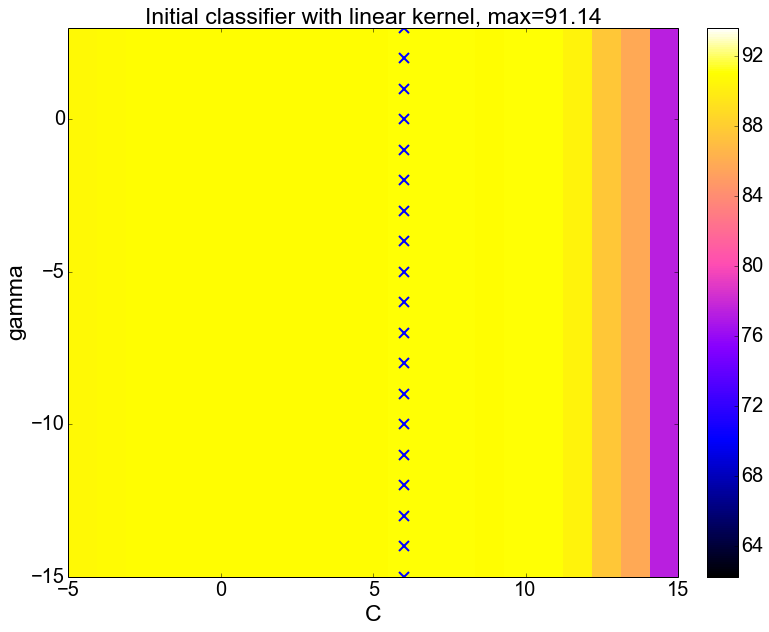
\includegraphics[width=1\textwidth]{plots/init_linear}
  \caption{Grid search over two-dimensional parameter space ($C$, $\gamma$) with linear kernel for the initial classifier. The maximal accuracy in 5-fold cross-validation is equal to 91.14 and is found for $log_{10}C=6$}
  \label{fig:initial_linear}
\end{figure}
\begin{figure}
\centering
  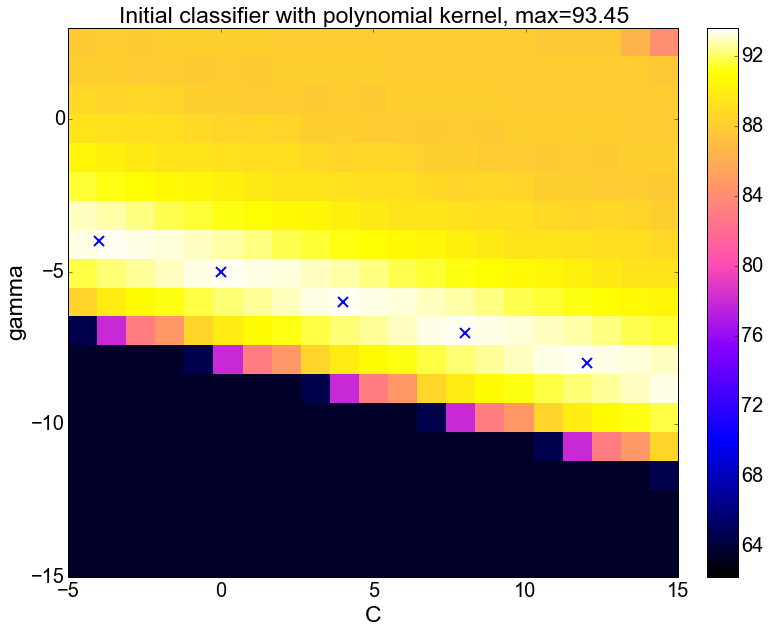
\includegraphics[width=1\textwidth]{plots/init_poly}
  \caption{Grid search over two-dimensional parameter space ($C$, $\gamma$) with polynomial $4^{th}$-degree kernel for the initial classifier. In the investigated interval there are 5 maxima. Classifier accuracy over 5-fold validation is equal to 93.45 and is found for instance for $log_{10}C=3$ and $log_{10}\gamma=-7$.}
  \label{fig:initial_poly}
\end{figure}

\begin{figure}
	\centering
  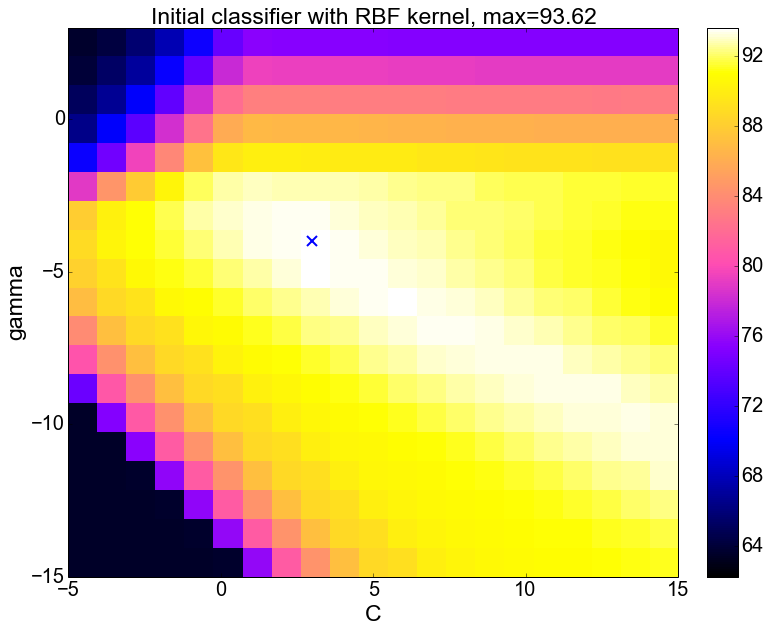
\includegraphics[width=1\textwidth]{plots/init_rbf}
   \caption{Grid search over two-dimensional parameter space ($C$, $\gamma$) with a radial-basis function kernel for the initial classifier. The maximal accuracy in 5-fold cross-validation is equal to 93.62 and is found for $log_{10}C=3$ and $log_{10}\gamma=-4$. This was the highest accuracy found in the first pass. The second pass refined the maximum around the initial result.}
   \label{fig:initial_rbf}
\end{figure}
\begin{figure}
	\centering
  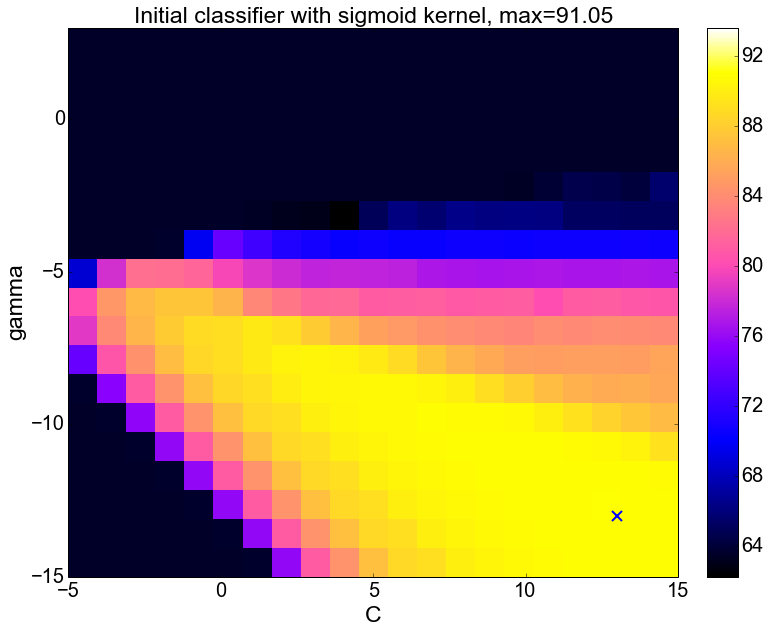
\includegraphics[width=1\textwidth]{plots/init_sigmoid}
  \caption{Grid search over two-dimensional parameter space ($C$, $\gamma$) with a sigmoid kernel for the initial classifier. The maximal accuracy in 5-fold cross-validation is equal to 91.05 and is found for $log_{10}C=13$ and $log_{10}\gamma=-13$}

  \label{fig:initial_sigmoid}
\end{figure}
\begin{figure}
	\centering
  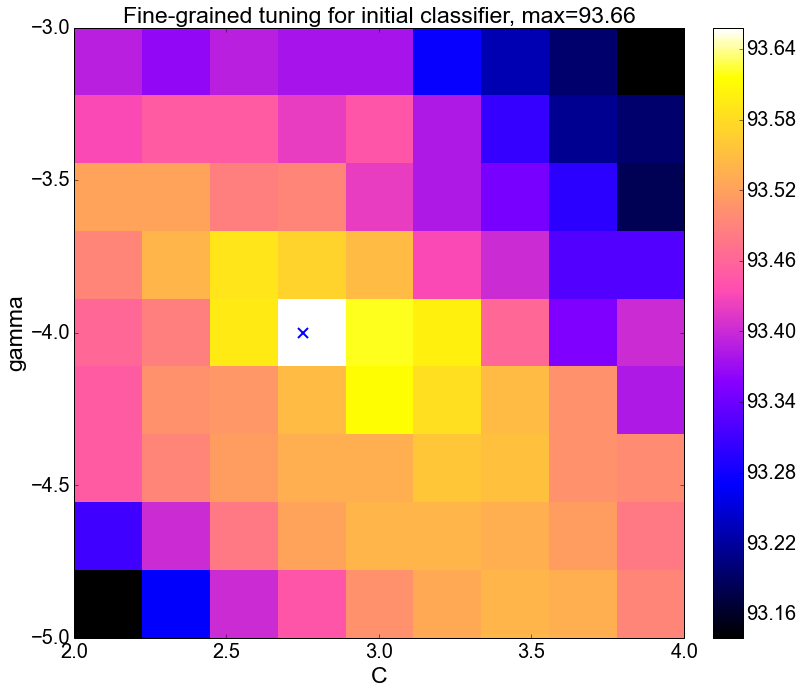
\includegraphics[width=\textwidth]{plots/init_fine}
  \caption{Fine-grain search around initial classifier with RBF kernel for the initial classifier (the color-mapping scheme is not coherent with the previous plots). Initial coarse-grain search yielded the maximum in ($log_{10}C=3$, $log_{10}\gamma=-4$) equal to 93.62. This search refines the search with $log_{10}step=0.25$ yielding maximum in ($log_{10}C=2.75$, $log_{10}\gamma=-4$) equal to 93.66. This parameters are used for training of the final classifier.}
  \label{fig:initial_fine}
\end{figure}
\begin{figure}
	\centering
  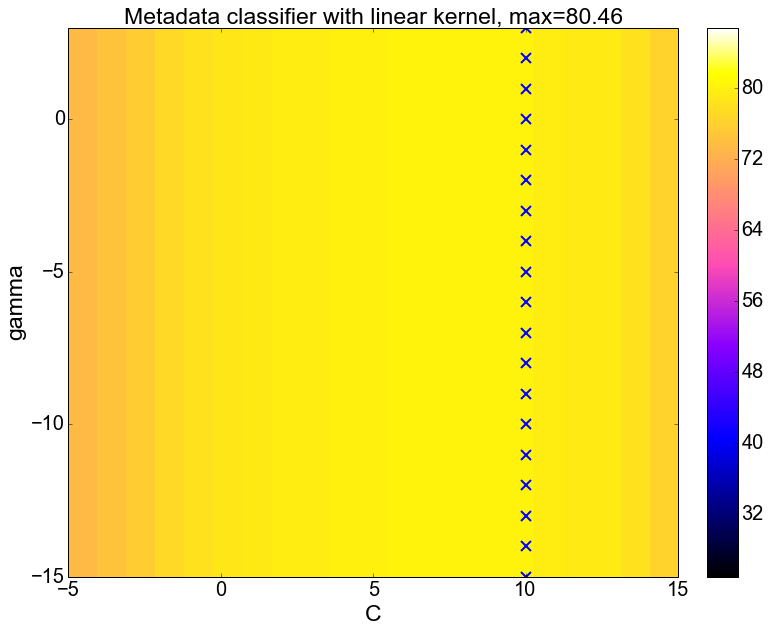
\includegraphics[width=\textwidth]{plots/meta_linear}
  \caption{Grid search over two-dimensional parameter space ($C$, $\gamma$) with linear kernel for the metadata classifier. The maximal accuracy in 5-fold cross-validation is equal to 80.46 and is found for $log_{10}C=19$}
  \label{fig:meta_linear}
\end{figure}
\begin{figure}
\centering
  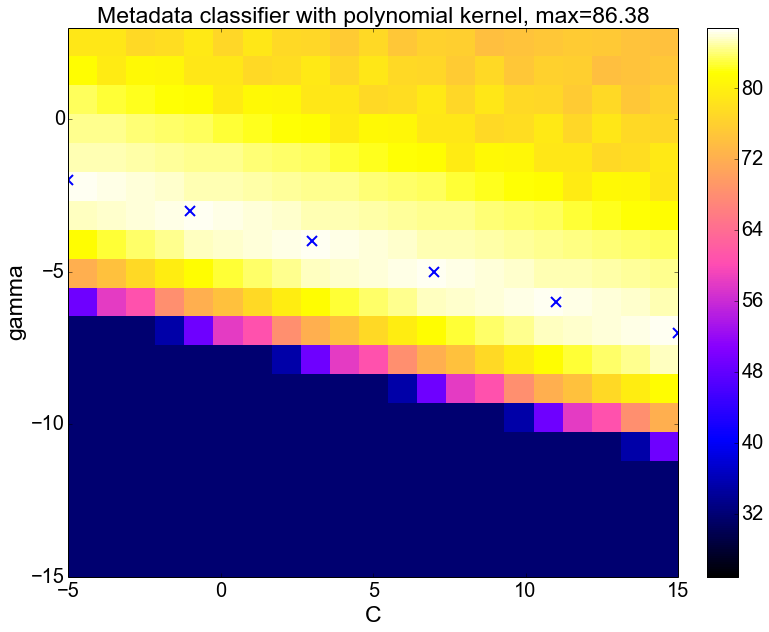
\includegraphics[width=\textwidth]{plots/meta_poly}
  \caption{Grid search over two-dimensional parameter space ($C$,$\gamma$) with polynomial $4^{th}$-degree kernel for the metadata classifier. In the investigated interval there are 5 maxima. Classifier accuracy over 5-fold validation is equal to 86.38 and is found for instance for $log_{10}C=7$ and $log_{10}\gamma=-5$.}
  \label{fig:meta_poly}
\end{figure}

\begin{figure}
	\centering
  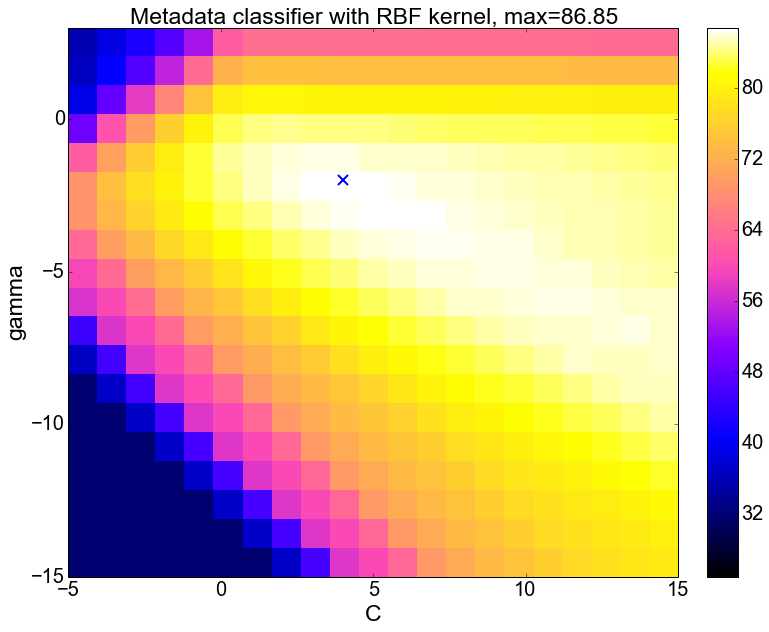
\includegraphics[width=\textwidth]{plots/meta_rbf}
   \caption{Grid search over two-dimensional parameter space ($C$, $\gamma$) with a radial-basis function kernel for the metadata classifier. The maximal accuracy in 5-fold cross-validation is equal to 86.85 and is found for $log_{10}C=4$ and $log_{10}\gamma=-2$. This was the highest accuracy found in the first pass. The second pass refined the maximum around the initial result.}
  \label{fig:meta_rbf}
\end{figure}
\begin{figure}
	\centering
  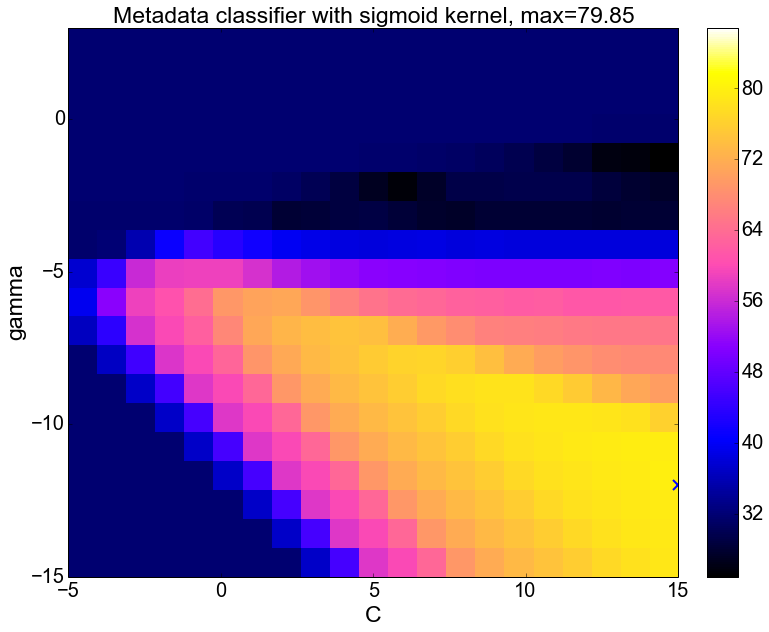
\includegraphics[width=\textwidth]{plots/meta_sigmoid}
  \caption{Grid search over two-dimensional parameter space ($C$, $\gamma$) with a sigmoid kernel for the initial classifier. The maximal accuracy in 5-fold cross-validation is equal to 79.85 and is found for $log_{10}C=15$ and $log_{10}\gamma=-12$}
  \label{fig:meta_sigmoid}
\end{figure}
\begin{figure}
	\centering
  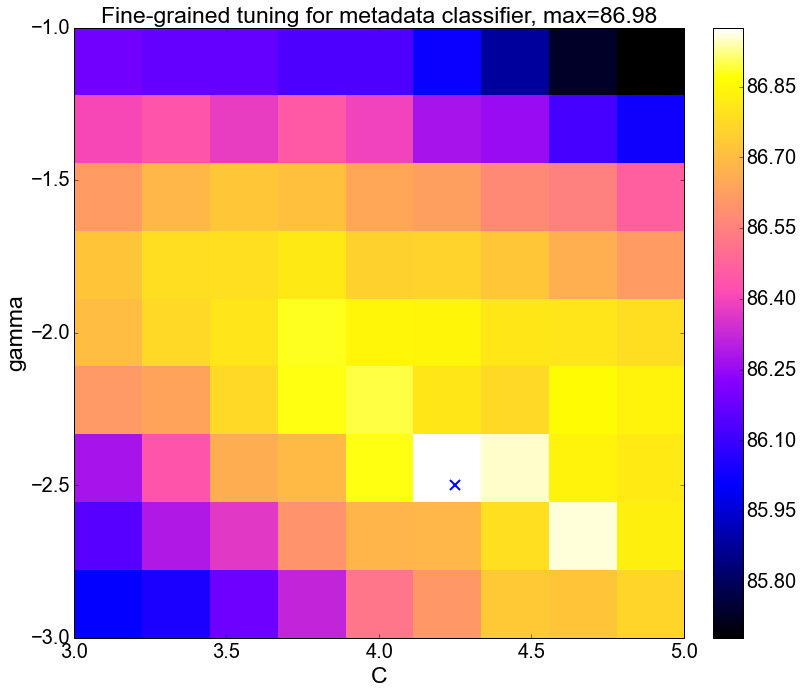
\includegraphics[width=\textwidth]{plots/meta_fine}
  \caption{Fine-grain search around initial classifier with RBF kernel for the metadata classifier (the color-mapping scheme is not coherent with the previous plots). Initial coarse-grain search yielded the maximum in ($log_{10}C=4$, $log_{10}\gamma=-2$) equal to 86.85. This search refines the search with $log_{10}step=0.25$ yielding maximum in ($log_{10}C=4.25$, $log_{10}\gamma=-2.5$) equal to 86.98. This parameters are used for training of the final classifier.}
  \label{fig:meta_fine}
\end{figure}
\end{center}

\subsection{Training of the final classifier}
After the optimal parameters have been found using a grid search, we train the classifiers to perform the final evaluation. This process is characterized in the appendix \ref{appendix:training_workflow}. To this end, we used classes \verb+SVMInitialZoneClassificationEvaluator+ and \verb+SVMMetadataClassificationEvaluator+ that build the classifier and perform cross-validation at a time. Its results are presented in the chapter \ref{chapter:evaluation}.

\section{Feature selection}
In both stages of classification we employed a set of features including almost one hundred elements. In appendix \ref{appendix:features} there is a detailed description of how their values are calculated. Briefly, they can be divided into following groups:

\subsubsection{Sequence features}
This group contains only two features: \textit{PreviousZoneFeature} and \textit{LastButOneZoneFeature}. It leverages the fact that the zones are classified after the process of reading order resolution is done. The features contain numerical value of two previous labels. In turn, this allows to incorporate sequence information into classification, which is not done in SVM by design (as opposed to for instance Hidden Markov Model).

\subsubsection{Formatting features}
This group of features contains information about graphical properties of text. It can be very helpful since certain elements in scholarly publications are usually typed with bigger font size.

\subsubsection{Layout features}
These features encode information about graphical layout on the page. This includes properties of the zone itself (e.g. \textit{WidthFeature}, \textit{HeightFeature}, \textit{LineMeanWidthFeature}) as well as features of the area between text zones (e.g. \textit{HorizontalRelativeProminenceFeature},\textit{VerticalRelativeProminenceFeature}, \textit{IsHighestOnThePage}, \textit{IsGreatestOnThePage}, \textit{DistanceFromNearestNeighbourFeature}).

\subsubsection{Semantic features}
This group of features encodes appearence of certain key-words that very often characterize certain parts of articles written with scientific english, e.g. \textit{keywords}, \textit{terms}, \textit{distributed}, \textit{reproduction}, \textit{open}, \textit{commons}, \textit{license}, \textit{creative}, \textit{copyright}, \textit{cited}, \textit{distribution}, \textit{access}, \textit{references}, \textit{author}, \textit{bibliography}, \textit{figure}, \textit{table}, \textit{editor}, \textit{email}, \textit{correspondence}, \textit{address}, \textit{abstract}, \textit{author details}, \textit{university}, \textit{department}, \textit{school}, \textit{institute}, \textit{affiliation}, \textit{affiliation}, \textit{research article}, \textit{review article}, \textit{editorial}, \textit{review}, \textit{debate}, \textit{case report}, \textit{research}, \textit{original research}, \textit{methodology}, \textit{clinical study}, \textit{commentary}, \textit{article}, 
 \textit{hypothesis}.

\subsubsection{Special features}
This group contains features that do not fit other groups described above. This includes e.g. \textit{IsAnywhereElseFeature}, \text{BracketCountFeature}, \text{CharCountFeature}, \text{CommaCountFeature}.